\pdfoutput=1
\pdfcompresslevel=9
\pdfinfo
{
    /Author ()
    /Title ()
    /Subject ()
    /Keywords ()
}

%\newcommand*{\memfontfamily}{pnc}
%\newcommand*{\memfontpack}{newcent}
\documentclass[a4paper,onecolumn,oneside,12pt]{memoir}
% Wydruk do archiwum
%\documentclass[a4paper,onecolumn,twoside,10pt]{memoir} 
%\renewcommand{\normalsize}{\fontsize{8pt}{10pt}\selectfont}

\usepackage[utf8]{inputenc}
\usepackage[T1]{fontenc}
\usepackage[polish]{babel}
\usepackage{setspace}
\usepackage{tabularx}
\usepackage{color,calc}
%\usepackage{soul} % pakiet z komendami do podkreœlania tekstu
%\usepackage{fourier} % pakiet zmieniaj¹cy czcionki na utopia
\usepackage{times} % pakiet zmieniaj¹cy czcionki na times 

%\usepackage{longtable}
%\usepackage{ltxtable}
%\usepackage{tabulary}

%%%%%% Ustawienia odpowiedzialne za sposób ³amania dokumentu
%\hyphenpenalty=10000		% nie dziel wyrazów zbyt czêsto
\clubpenalty=10000      %kara za sierotki
\widowpenalty=10000  % nie pozostawiaj wdów
\brokenpenalty=10000		% nie dziel wyrazów miêdzy stronami
\exhyphenpenalty=999999		% nie dziel s³ów z myœlnikiem
\righthyphenmin=3			% dziel minimum 3 litery

%\tolerance=4500
%\pretolerance=250
%\hfuzz=1.5pt
%\hbadness=1450

%ustawienia rozmiarów: tekstu, stopki, marginesów 
\setlength{\textwidth}{\paperwidth}
\addtolength{\textwidth}{-5cm}
\setlength{\textheight}{\paperheight}
\addtolength{\textheight}{-5cm}
\setlength{\oddsidemargin}{-0.04cm} % domyœlnie jest 1 cal = 2.54 cm, st¹d -0.04 da margines 2.5cm
\setlength{\evensidemargin}{-0.04cm} % domyœlnie jest 1 cal = 2.54 cm, st¹d -0.04 da margines 2.5cm
\topmargin -1.25cm
\footskip 1.4cm 

\linespread{1.3}

\usepackage{ifpdf}
%\newif\ifpdf \ifx\pdfoutput\undefined
%\pdffalse % we are not running PDFLaTeX
%\else
%\pdfoutput=1 % we are running PDFLaTeX
%\pdftrue \fi
\ifpdf
\usepackage[pdftex]{graphicx,hyperref}
\DeclareGraphicsExtensions{.pdf,.jpg,.mps,.png}
\pdfcompresslevel=9
\else
\usepackage{graphicx}
\DeclareGraphicsExtensions{.eps,.ps,.jpg,.mps,.png}
\fi
\sloppy

%\graphicspath{{rys01/}{rys02/}}

\renewcommand{\topfraction}{0.95}
\renewcommand{\bottomfraction}{0.95}
\renewcommand{\textfraction}{0.05}
\renewcommand{\floatpagefraction}{0.35}


%%%%%%%%%%%%%%%%%%%%%%%%%%%%%%%%%%%%%%%
%                  Definicja strony tytu³owej 
%%%%%%%%%%%%%%%%%%%%%%%%%%%%%%%%%%%%%%%
\makeatletter
%Uczelnia
\newcommand\uczelnia[1]{\renewcommand\@uczelnia{#1}}
\newcommand\@uczelnia{}
%Wydzia³
\newcommand\wydzial[1]{\renewcommand\@wydzial{#1}}
\newcommand\@wydzial{}
%Kierunek
\newcommand\kierunek[1]{\renewcommand\@kierunek{#1}}
\newcommand\@kierunek{}
%SpecjalnoϾ
\newcommand\specjalnosc[1]{\renewcommand\@specjalnosc{#1}}
\newcommand\@specjalnosc{}
%Tytu³ po angielsku
\newcommand\titleEN[1]{\renewcommand\@titleEN{#1}}
\newcommand\@titleEN{}
%Tytu³ krótki
\newcommand\titleShort[1]{\renewcommand\@titleShort{#1}}
\newcommand\@titleShort{}
%Promotor
\newcommand\promotor[1]{\renewcommand\@promotor{#1}}
\newcommand\@promotor{}

\def\maketitle{%
  \null
  \pagestyle{empty}%
	{\centering\vspace{-1cm}
		{\fontsize{22pt}{24pt}\selectfont \@uczelnia}\\[0.4cm]
		{\fontsize{22pt}{24pt}\selectfont \@wydzial }\\[0.5cm]
		\hrule \vspace*{0.7cm}
	}
{\flushleft\fontsize{14pt}{16pt}\selectfont%
\begin{tabular}{ll}
Kierunek: & \@kierunek\\
Specjalność & \@specjalnosc\\
\end{tabular}\\[1.3cm]
}
{\centering
%{\fontsize{24pt}{26pt}\selectfont PRACA DYPLOMOWA}\\[0.5cm]
%{\fontsize{24pt}{26pt}\selectfont MAGISTERSKA}\\[2cm]
{\fontsize{24pt}{26pt}\selectfont Projekt Inżynierski}\\[1.5cm]
}
%
\begin{tabularx}{\linewidth}{p{6cm}>{\centering\arraybackslash}X}
		&{\fontsize{16pt}{18pt}\selectfont \@title}\\[5mm] 	%UWAGA: tutaj jest miejsce na tyty³ w jêzyku polskim
		&{\fontsize{16pt}{18pt}\selectfont \@titleEN}\\[10mm] %UWAGA: tutaj jest miejsce na tyty³ w jêzyku angielskim
\end{tabularx}
\vfill
\begin{tabularx}{\linewidth}{p{6cm}l}
		%UWAGA: tutaj jest miejsce na autora pracy
		&{\fontsize{16pt}{18pt}\selectfont Autor:}\\[5mm]
		&{\fontsize{14pt}{16pt}\selectfont \@author}\\[10mm]
		%UWAGA: tutaj jest miejsce na promotora pracy
		&{\fontsize{16pt}{18pt}\selectfont Prowadzący pracę:}\\[5mm]
		&{\fontsize{14pt}{16pt}\selectfont \@promotor}\\[10mm]
		&{\fontsize{16pt}{18pt}\selectfont Ocena pracy:}\\[20mm]
	\end{tabularx}
\hrule\vspace*{0.3cm}
{\centering
%{\fontsize{24pt}{26pt}\selectfont PRACA DYPLOMOWA}\\[0.5cm]
%{\fontsize{24pt}{26pt}\selectfont MAGISTERSKA}\\[2cm]
{\fontsize{16pt}{18pt}\selectfont \@date}\\[0cm]
}
\normalfont
 \cleardoublepage
}
\makeatother
%%%%%%%%%%%%%%%%%%%%%%%%%%%%%%%%%%%%%%%
%                  Styl rozdzia³ów 
%%%%%%%%%%%%%%%%%%%%%%%%%%%%%%%%%%%%%%%
\setcounter{secnumdepth}{3}
\setcounter{tocdepth}{3}
%\definecolor{niceblue}{rgb}{.168,.234,.671}

%\AtBeginDocument{% 
        \addto\captionspolish{% 
        \renewcommand{\tablename}{Tab.}% 
}%} 

%\AtBeginDocument{% 
%        \addto\captionspolish{% 
%        \renewcommand{\chaptername}{Rozdzia³}% 
%}} 

%\AtBeginDocument{% 
        \addto\captionspolish{% 
        \renewcommand{\figurename}{Rys.}% 
}%}
        \addto\captionspolish{% 
        \renewcommand{\bibname}{Literatura}% 
}

%%%%%%%%%%%%%%%%%%%%%%%%%%%%%%%%%%%%%%%%%%%%%%%%%%%%%%%%%%%%%%%%%%                  Styl wyliczenia (opis skrótów) 
%%%%%%%%%%%%%%%%%%%%%%%%%%%%%%%%%%%%%%%%%%%%%%%%%%%%%%%%%%%%%%%%%
\newenvironment{Ventry}[1]%
 {\begin{list}{}{\renewcommand{\makelabel}[1]{\textbf{##1}\hfill}%
   \settowidth{\labelwidth}{\textbf{#1}}%
   \setlength{\leftmargin}{3cm}}}%
 {\end{list}}

\addtopsmarks{headings}{%
\nouppercaseheads % added at the beginning
}{%
\createmark{chapter}{both}{shownumber}{}{. \space}
%\createmark{chapter}{left}{shownumber}{}{. \space}
\createmark{section}{right}{shownumber}{}{. \space}
}%use the new settings
\pagestyle{headings}

\newlength\mytemplengtha

\setcounter{secnumdepth}{2}
\setcounter{tocdepth}{2}
\setsecnumdepth{subsection} % activating subsubsec numbering in doc

\makeatletter
\copypagestyle{outer}{headings}
\makeoddhead{outer}{}{}{\slshape\rightmark}
\makeevenhead{outer}{\slshape\leftmark}{}{}
\makeoddfoot{outer}{\@author:~\@titleShort}{}{\thepage}
\makeevenfoot{outer}{\thepage}{}{\@author:~\@title}
\makeheadrule{outer}{\linewidth}{\normalrulethickness}
\makefootrule{outer}{\linewidth}{\normalrulethickness}{6pt}
\makeatother

% fix plain
%\copypagestyle{plain}{outer} % overwrite plain with outer
\makeoddhead{plain}{}{}{} % remove right header
\makeevenhead{plain}{}{}{} % remove left header
\makeevenfoot{plain}{}{}{}
\makeoddfoot{plain}{}{}{}

%\copypagestyle{plain}{outer} % overwrite plain with outer
\makeoddhead{empty}{}{}{} % remove right header
\makeevenhead{empty}{}{}{} % remove left header
\makeevenfoot{empty}{}{}{}
\makeoddfoot{empty}{}{}{}

\pagestyle{outer}


\makeatletter
\def\@seccntformat#1{\csname the#1\endcsname.\quad}
\def\numberline#1{\hb@xt@\@tempdima{#1\if&#1&\else.\fi\hfil}}
\makeatother

\renewcommand{\chapternumberline}[1]{#1.\quad}
\renewcommand{\cftchapterdotsep}{\cftdotsep}

\begin{document}
\title{Internetowy system wspomagania treningów    aerobowych z aplikacją mobilną}
\titleShort{Internetowy system wspomagania ...}
\titleEN{Internet system for aerobic training with a mobile application}
\author{Jacek Wieczorek}
\uczelnia{Politechnika Wrocławska}
\wydzial{Wydział Elektroniki}
\kierunek{Informatyka}
\specjalnosc{Inżynieria Internetowa}
\promotor{dr inż. Tomasz Walkowiak}
\date{Wrocław, 2012}
\maketitle

\pagestyle{outer}

\tableofcontents


\chapter{Wprowadzenie}

\section{Cel pracy}
\label{sec:cel_pracy}
\paragraph{}
Celem niniejszego projektu inżynierskiego jest zaprojektowanie oraz zaimplementowanie systemu do wspomagania treningów areobowych. Główną częścią systemu jest aplikacja internetowa wspomagana przez aplikację mobilną. By zapewnić możliwość przesyłania danych do serwera, konieczne jest stworzenie API, będącego pośrednikiem między aplikacją mobilną, a bazą danych.
System ma pozwolić użytkownikom zarządzać treningami, prezentować swoje osiągnięcia innym osobom korzystjącym z portalu i swobodnie komunikować się z nimi.
% paragraph  (end)
\paragraph{} % (fold)
\label{par:}
Podstawowe wymagania, które ma spełniać projekt :
\begin{itemize}
	\item Tworzenie i edycja treningów
	\item Tworzenie i edycja profili użytkowników
	\item Komunikacja pomiędzy użytkownikami
	\item Synchronizacja danych z aplikacji mobilnej
	\item Zarządzanie prywatnością profilu użytkownika
	\item Możliwość przeglądania treningów innych użytkowników
	\item Stworzenie formy małego portalu społecznościowego
\end{itemize}
% paragraph  (end)

\section{Istniejące rozwiązania}
\paragraph{}
Na rynku dostępne jest wiele rozwiązań pozwalających na zarządzanie treningami. Jednak większość z nich jest aplikacjami komercyjnymi, których darmowe produkty obarczone są dużą liczbą reklam lub ograniczoną liczbą dostępnych funckcjonalności. Ponadto aplikacje te często zatraciły swoją idę wspierania treningów i stały się kolejnymi portalami typu Social Media. Celem tego projektu jest stworzenie systemu, oferującego podobne możliwośći jak oferowane na rynku rozwiązania, nie tracąc przy tym na prostocie użytkowania i przejrzystościu interfejsu użytkownika.

\chapter{Opis systemu i komponenty wykorzystywane w projekcie}
\label{cha:projektsys}

\section{Projekt systemu} % (fold)
\label{sec:projket_systemu}
W celu otrzymania w pełni działającego systemu, należy w odpowiedni sposób synchronizować pracę trzech kluczowych elementów:
\begin{itemize}
	\item aplikacja internetowa - warstwa prezentacji systemu,
	\item aplikacja mobilna z bazą danych SQLite - wspomaganie aplikacji internetowej w gromadzeniu danych,
	\item REST Api - umożliwienie przesyłania danych z aplikacji mobilnej do bazy danych.
\end{itemize}

\paragraph{} % (fold)
\label{par:}
Ogólny schemat całego systemu pokazany został na rysunku \ref{fig:system_schema}. Aplikacja internetowa napisana została w języku C\# działającym na platformie .NET z wykorzystaniem frameworka ASP.NET MVC 3. Moduł odpowiedzialny za implementację REST Api również wykorzystuje język C\# i popularną w świecie .NET platformę do tworzenia WebService'ów - Windows Communication Foundation. Aplikacja mobilna napisana została natomiast w języku Java i działa na systemie operacyjnym Android. Szczegółowy opis wykorzystanych technologii wraz z odnośnikami do literatury zamieszczony został w Sekcjach od \ref{sec:jezyk} do \ref{sec:inne_biblioteki_wykorzystane_w_projekcie}. W rozdziałach od \ref{cha:webapp} do \ref{cha:restapi} znajdują się dokładne opisy przedstawionych modułów. W sekcji \ref{sec:in_ynieria_wymaga_} umieszczona została pełna lista wymagań dostycząca poszczególnych elementów systemu.
% paragraph  (end)

% section projket_systemu (end)

\begin{figure}[ht]
	\centering
		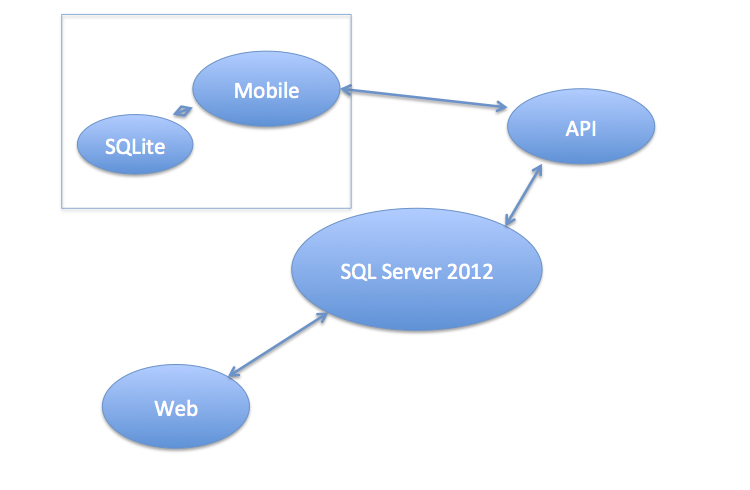
\includegraphics[width=1\linewidth]{assets/system_schema.png}
	\caption{Schemat zaprojektowanego systemu}
	\label{fig:system_schema}
\end{figure}


\section{Inżynieria wymagań} % (fold)
\label{sec:in_ynieria_wymaga_}
Sekcje przedstawionne poniżej opsiują wymagania, jakie zostały nałożone na projekt. Wszytskie wymienione niżej funkcjonalności zostały zaimplementowane.

\subsection{Apliakcja intenetowa} % (fold)
\label{sub:apliakcja_intenetowa}
\subsubsection{Wymagania funkcjonalne}
\begin{center}
      \begin{tabular}{rp{10cm}}
	      \multicolumn{2}{l}{\textbf{Rejestracja użytkowników}} \\
	      \hline
	      ID: & FUN1 \\
	      Opis: & Aplikacja umożliwia rejestrację użytkowników z podaniem unikalnej nazwy użytkownika, adresu email, hasła, imienia i nazwiska, daty urodzenia. \\
	      Priorytet: & wymagane \\
	      Powiązania: & --- \\
    \end{tabular}
\end{center}

\begin{center}
      \begin{tabular}{rp{10cm}}
	      \multicolumn{2}{l}{\textbf{Logowanie użytkowników}} \\
	      \hline
	      ID: & FUN2 \\
	      Opis: & Aplikacja umożliwia logowanie użytkowników poprzez podanie prawidłowego loginu i hasła \\
	      Priorytet: & wymagane \\
	      Powiązania: & FUN1 \\
    \end{tabular}
\end{center}

\begin{center}
      \begin{tabular}{rp{10cm}}
	      \multicolumn{2}{l}{\textbf{Wyświetlanie treningów}} \\
	      \hline
	      ID: & FUN3 \\
	      Opis: & Aplikacja umożliwia agregowanie treningów poprzez wyświetlenie ich na kalendarzu \\
	      Priorytet: & wymagane \\
	      Powiązania: & --- \\
    \end{tabular}
\end{center}

\begin{center}
      \begin{tabular}{rp{10cm}}
	      \multicolumn{2}{l}{\textbf{Szczegółowy widok treningu}} \\
	      \hline
	      ID: & FUN4 \\
	      Opis: & Aplikacja pozwala na wyświetlenie szczegółowych danych dotyczących treningu wraz z widokiem zaznaczonej na mapie przebytej trasy \\
	      Priorytet: & wymagane \\
	      Powiązania: & FUN3\\
    \end{tabular}
\end{center}

\begin{center}
      \begin{tabular}{rp{10cm}}
	      \multicolumn{2}{l}{\textbf{Tworzenie treningu z podstawowymi danymi}} \\
	      \hline
	      ID: & FUN5 \\
	      Opis: & Aplikacja pozwala na dodanie treningu z podstawowymi danymi : typ treningu, czas rozpoczęcia i zakończenia,	 przebyty dystans \\
	      Priorytet: & wymagane \\
	      Powiązania: & FUN3 \\
    \end{tabular}
\end{center}

\begin{center}
      \begin{tabular}{rp{10cm}}
	      \multicolumn{2}{l}{\textbf{Wyświetlanie profilu użytkownika}} \\
	      \hline
	      ID: & FUN6 \\
	      Opis: & Aplikacja pozwala na wyświetlenie profilu użytkowników \\
	      Priorytet: & wymagane \\
	      Powiązania: & --- \\
    \end{tabular}
\end{center}

\begin{center}
      \begin{tabular}{rp{10cm}}
	      \multicolumn{2}{l}{\textbf{Edycja profilu użytkownika}} \\
	      \hline
	      ID: & FUN7 \\
	      Opis: & Aplikacja pozwala na edytowanie profilu użytkowników \\
	      Priorytet: & wymagane \\
	      Powiązania: & FUN6 \\
    \end{tabular}
\end{center}

\begin{center}
      \begin{tabular}{rp{10cm}}
	      \multicolumn{2}{l}{\textbf{Profil prywatny}} \\
	      \hline
	      ID: & FUN7 \\
	      Opis: & Aplikacja pozwala na ukrycie częsci danych wyświetlanych na profilu \\
	      Priorytet: & wymagane \\
	      Powiązania: & FUN6 \\
    \end{tabular}
\end{center}

\begin{center}
      \begin{tabular}{rp{10cm}}
	      \multicolumn{2}{l}{\textbf{Ukrywanie treningów}} \\
	      \hline
	      ID: & FUN9 \\
	      Opis: & Aplikacja pozwala na pokazywanie treningów wszytskim użytkownikom, użytkownikom, którzy za mną podążają, tylko właścicielowi profilu \\
	      Priorytet: & wymagane \\
	      Powiązania: & FUN3 \\
    \end{tabular}
\end{center}

\begin{center}
      \begin{tabular}{rp{10cm}}
	      \multicolumn{2}{l}{\textbf{Podążanie za użytkownikami}} \\
	      \hline
	      ID: & FUN10 \\
	      Opis: & Aplikacja pozwala na podążanie za użytkownikami \\
	      Priorytet: & wymagane \\
	      Powiązania: & FUN3 \\
    \end{tabular}
\end{center}

\begin{center}
      \begin{tabular}{rp{10cm}}
	      \multicolumn{2}{l}{\textbf{Wysyłanie wiadmości}} \\
	      \hline
	      ID: & FUN11 \\
	      Opis: & Aplikacja pozwala na wysyłanie wiadomości pomiędzy użytkownikami \\
	      Priorytet: & wymagane \\
	      Powiązania: & FUN3 \\
    \end{tabular}
\end{center}

\begin{center}
      \begin{tabular}{rp{10cm}}
	      \multicolumn{2}{l}{\textbf{Tablica ogłoszeń}} \\
	      \hline
	      ID: & FUN12 \\
	      Opis: & Aplikacja pozwala na wyświetlanie informacji o aktywnościach podążanych użytkowników \\
	      Priorytet: & niewymagane \\
	      Powiązania: & FUN3 \\
    \end{tabular}
\end{center}

\begin{center}
      \begin{tabular}{rp{10cm}}
	      \multicolumn{2}{l}{\textbf{Lokalizacja}} \\
	      \hline
	      ID: & FUN13 \\
	      Opis: & Aplikacja pozwala na wielojęzykowość\\
	      Priorytet: & niewymagane \\
	      Powiązania: & --- \\
    \end{tabular}
\end{center}

\subsubsection{Wymagania niefunkcjonalne}
 \begin{center}
    \begin{tabular}{rp{10cm}}
      \multicolumn{2}{l}{\textbf{Interfejs WWW}} \\
      \hline
      ID: & NFUN1 \\
      Opis: & Aplikacja ma posiadać interfejs WWW. \\
      Priorytet: & wymagane \\
      Powiązania: & --- \\
    \end{tabular}
    \end{center}

\subsubsection{Wymagania bezpieczeństwa}
\begin{center}
      \begin{tabular}{rp{10cm}}
	      \multicolumn{2}{l}{\textbf{Autoryzacja użytkowników}} \\
	      \hline
	      ID: & SEC1 \\
	      Opis: & Aplikacja powinna umożliwiać dostęp do informacji tylko zalogowanym użytkownikom \\
	      Priorytet: & wymagane \\
	      Powiązania: & --- \\
    \end{tabular}
\end{center}

\begin{center}
      \begin{tabular}{rp{10cm}}
	      \multicolumn{2}{l}{\textbf{Odporność na SQL Injection}} \\
	      \hline
	      ID: & SEC2 \\
	      Opis: & Aplikacja powinna uniemożliwiać ataki typu SQL Injection \\
	      Priorytet: & wymagane \\
	      Powiązania: & --- \\
    \end{tabular}
\end{center}

\begin{center}
      \begin{tabular}{rp{10cm}}
	      \multicolumn{2}{l}{\textbf{Przechowywanie hasła}} \\
	      \hline
	      ID: & SEC3 \\
	      Opis: & Aplikacja powinna uniemożliwić złamanie hasła popularnymi metodami : brutal force, atak słownikowy, atak z wykorzystaniem tablic tęczowych \\
	      Priorytet: & wymagane \\
	      Powiązania: & --- \\
    \end{tabular}
\end{center}

\subsubsection{Wymagania technologiczne}
      \begin{center}
      \begin{tabular}{rp{10cm}}
        \multicolumn{2}{l}{\textbf{C\#, CoffeeScript, HTML5, CSS3}} \\
        \hline
        ID: & TEC1 \\
        Opis: & Aplikacja powinna zostać napisana w języku C\# z wykorzystaniem języków CoffeeScript, HTML5, CSS3 \\
        Priorytet: & wymagane \\
        Powiązania: & --- \\
      \end{tabular}
      \end{center}

      \begin{center}
      \begin{tabular}{rp{10cm}}
        \multicolumn{2}{l}{\textbf{ASP.NET MVC 3}} \\
        \hline
        ID: & TEC2 \\
        Opis: & Aplikacja powinna zostać stworzona wykorzsytaując framework ASP.NET MVC 3 \\
        Priorytet: & wymagane \\
        Powiązania: & TEC1 \\
      \end{tabular}
      \end{center}



      \begin{center}
      \begin{tabular}{rp{10cm}}
        \multicolumn{2}{l}{\textbf{Baza danych}} \\
        \hline
        ID: & TEC3 \\
        Opis: & Aplikacja powinna wykorzystywać bazę Microsoft SQL Server 2012. \\
        Priorytet: & wymagane \\
        Powiązania: & --- \\
      \end{tabular}
      \end{center}



      \begin{center}
      \begin{tabular}{rp{10cm}}
        \multicolumn{2}{l}{\textbf{Windows Azure}} \\
        \hline
        ID: & TEC4 \\
        Opis: & Aplikacja powinna być przystosowana do platformy Windows Azure \\
        Priorytet: & niewymagane \\
        Powiązania: & --- \\
      \end{tabular}
      \end{center}

\subsection{Aplikacja mobilna} % (fold)
\subsubsection{Wymagania funkcjonalne}
\label{sub:aplikacja_mobilna}
\begin{center}
      \begin{tabular}{rp{10cm}}
	      \multicolumn{2}{l}{\textbf{Rejestrowanie przebytej trasy}} \\
	      \hline
	      ID: & FUN14 \\
	      Opis: & Aplikacja pozwala na rejestrowanie przebytej trasy zapomocą odbiornika GPS i zapisywanie w bazie danych \\
	      Priorytet: & wymagane \\
	      Powiązania: & --- \\
    \end{tabular}
\end{center}

\begin{center}
      \begin{tabular}{rp{10cm}}
	      \multicolumn{2}{l}{\textbf{Logowanie}} \\
	      \hline
	      ID: & FUN15 \\
	      Opis: & Aplikacja pozwala na zalogowanie się przez wysłanie żądania do REST API \\
	      Priorytet: & wymagane \\
	      Powiązania: & --- \\
    \end{tabular}
\end{center}

\begin{center}
      \begin{tabular}{rp{10cm}}
	      \multicolumn{2}{l}{\textbf{Rejestrowanie danych dotyczących treningu}} \\
	      \hline
	      ID: & FUN16 \\
	      Opis: & Aplikacja pozwala na zapisanie w bazie danych podstawowych informacji dotyczących treningu: data rozpoczęcia i zakończenia, typ treningu, przebyty dystans  \\
	      Priorytet: & wymagane \\
	      Powiązania: & FUN13 \\
    \end{tabular}
\end{center}

\begin{center}
      \begin{tabular}{rp{10cm}}
	      \multicolumn{2}{l}{\textbf{Wyświetlanie aktualnych danych dotyczących trwającego treningu}} \\
	      \hline
	      ID: & FUN17 \\
	      Opis: & Aplikacja pozwala na wyświetlenie czasu trwania trenigu i przebytego dystansu w czasie rzeczywistym \\
	      Priorytet: & wymagane \\
	      Powiązania: & --- \\
    \end{tabular}
\end{center}

\begin{center}
      \begin{tabular}{rp{10cm}}
	      \multicolumn{2}{l}{\textbf{Wysyłanie danych}} \\
	      \hline
	      ID: & FUN18 \\
	      Opis: & Aplikacja pozwala na wysyłąnie danych do REST API w celu zapisania ich w bazie danych na serwerze \\
	      Priorytet: & wymagane \\
	      Powiązania: & --- \\
    \end{tabular}
\end{center}
% subsection aplikacja_mobilna (end)

\subsubsection{Wymagania niefunkcjonalne}
 \begin{center}
    \begin{tabular}{rp{10cm}}
      \multicolumn{2}{l}{\textbf{Interfejs WWW}} \\
      \hline
      ID: & NFUN2 \\
      Opis: & Aplikacja ma posiadać graficzny interfejs użytkownika \\
      Priorytet: & wymagane \\
      Powiązania: & --- \\
    \end{tabular}
    \end{center}

\subsubsection{Wymagania bezpieczeństwa}
\begin{center}
      \begin{tabular}{rp{10cm}}
	      \multicolumn{2}{l}{\textbf{Autoryzacja użytkowników}} \\
	      \hline
	      ID: & SEC4 \\
	      Opis: & Aplikacja powinna umożliwiać dostęp do informacji tylko zalogowanym użytkownikom \\
	      Priorytet: & wymagane \\
	      Powiązania: & --- \\
    \end{tabular}
\end{center}

\begin{center}
      \begin{tabular}{rp{10cm}}
	      \multicolumn{2}{l}{\textbf{Autoryzacja za pomocą tokenu}} \\
	      \hline
	      ID: & SEC5 \\
	      Opis: & Aplikacja powinna autoryzować żądania za pomocą token  \\
	      Priorytet: & wymagane \\
	      Powiązania: & --- \\
    \end{tabular}
\end{center}

\subsubsection{Wymagania technologiczne}
      \begin{center}
      \begin{tabular}{rp{10cm}}
        \multicolumn{2}{l}{\textbf{Java}} \\
        \hline
        ID: & TEC5 \\
        Opis: & Aplikacja powinna zostać napisana w języku Java\\
        Priorytet: & wymagane \\
        Powiązania: & --- \\
      \end{tabular}
      \end{center}

      \begin{center}
      \begin{tabular}{rp{10cm}}
        \multicolumn{2}{l}{\textbf{Android}} \\
        \hline
        ID: & TEC6 \\
        Opis: & Aplikacja powinna działać na platformie Android \\
        Priorytet: & wymagane \\
        Powiązania: & TEC1 \\
      \end{tabular}
      \end{center}



      \begin{center}
      \begin{tabular}{rp{10cm}}
        \multicolumn{2}{l}{\textbf{Baza danych}} \\
        \hline
        ID: & TEC7 \\
        Opis: & Aplikacja ma wykorzystywać bazę Microsoft SQLite. \\
        Priorytet: & wymagane \\
        Powiązania: & --- \\
      \end{tabular}
      \end{center}



      \begin{center}
      \begin{tabular}{rp{10cm}}
        \multicolumn{2}{l}{\textbf{GPS}} \\
        \hline
        ID: & TEC8 \\
        Opis: & Aplikacja powinna obsługiwać odbiornik GPS \\
        Priorytet: & niewymagane \\
        Powiązania: & --- \\
      \end{tabular}
      \end{center}

\subsection{REST API} % (fold)
\subsubsection{Wymagania funkcjonalne}
\label{sub:aplikacja_mobilna}
\begin{center}
      \begin{tabular}{rp{10cm}}
	      \multicolumn{2}{l}{\textbf{Autoryzacja użytkowników}} \\
	      \hline
	      ID: & FUN19 \\
	      Opis: & API pozwala na autoryzowanie użytkowników aplikacji mobilnej \\
	      Priorytet: & wymagane \\
	      Powiązania: & --- \\
    \end{tabular}
\end{center}

\begin{center}
      \begin{tabular}{rp{10cm}}
	      \multicolumn{2}{l}{\textbf{Zapisywanie treningów}} \\
	      \hline
	      ID: & FUN12 \\
	      Opis: & API pozwala na zapisywanie treningów z aplikacji mobilnej w bazie danych na serwerze \\
	      Priorytet: & wymagane \\
	      Powiązania: & --- \\
    \end{tabular}
\end{center}

% subsection aplikacja_mobilna (end)

\subsubsection{Wymagania niefunkcjonalne}
 \begin{center}
    \begin{tabular}{rp{10cm}}
      \multicolumn{2}{l}{\textbf{Zewnętrzne metody}} \\
      \hline
      ID: & NFUN3 \\
      Opis: & Aplikacja ma posiadać dostępne pod postacią adresów URI metody \\
      Priorytet: & wymagane \\
      Powiązania: & --- \\
    \end{tabular}
    \end{center}

\subsubsection{Wymagania bezpieczeństwa}
\begin{center}
      \begin{tabular}{rp{10cm}}
	      \multicolumn{2}{l}{\textbf{Autoryzacja użytkowników}} \\
	      \hline
	      ID: & SEC4 \\
	      Opis: & Aplikacja powinna przetwarzać tylko autoryzowane żądania \\
	      Priorytet: & wymagane \\
	      Powiązania: & --- \\
    \end{tabular}
\end{center}


\subsubsection{Wymagania technologiczne}
      \begin{center}
      \begin{tabular}{rp{10cm}}
        \multicolumn{2}{l}{\textbf{C\#}} \\
        \hline
        ID: & TEC8 \\
        Opis: & Aplikacja powinna zostać napisana w języku C\#\\
        Priorytet: & wymagane \\
        Powiązania: & --- \\
      \end{tabular}
      \end{center}

      \begin{center}
      \begin{tabular}{rp{10cm}}
        \multicolumn{2}{l}{\textbf{Windows Communication Foundation}} \\
        \hline
        ID: & TEC9 \\
        Opis: & Aplikacja powinna działać z wykorzystaniem Windows Communication Foundation \\
        Priorytet: & wymagane \\
        Powiązania: & TEC1 \\
      \end{tabular}
      \end{center}

      \begin{center}
      \begin{tabular}{rp{10cm}}
        \multicolumn{2}{l}{\textbf{Baza danych}} \\
        \hline
        ID: & TEC10 \\
        Opis: & Aplikacja ma wykorzystywać bazę Microsoft SQLite. \\
        Priorytet: & wymagane \\
        Powiązania: & --- \\
      \end{tabular}
      \end{center}


\section{ C\# i .NET }
\label{sec:jezyk}
\paragraph{}
C\# \cite{csharp}  jest obiektowym językiem programowania stworzonym dla firmy Microsoft przez zespół Andersa Hejslberga. Język ten powstał jako alternatywa dla Javy. Programy napisane w C\# kompilowane są do natywnego języka Common Intermediate Language (CIL), czyli kodu pośredniego w środowisku takim jak .NET czy Mono.
\paragraph{}
.NET Framework jest platformą programistyczną obejmującą środowisko uruchomieniowe CLR (Common Language Runtime) oraz biblioteki klas z podstawowymi funkcjonalnościami. Zadaniem .NET jest zarządzanie elementami systemu, takimi jak: kod aplikacji, pamięć oraz zabezpieczenia. .NET umożliwia uruchamianie aplikacji zarówno na systemie, w którym istnieje działająca implementacja platformy oraz po stronie serwera IIS. Platforma .NET nie określa jednoznacznie języka programowania. Aplikacje działające przy wykorzystaniu platformy .NET mogą być napisane w C\#, F\#, J\#, VB.NET, C++/CLI czy Delphi 8. 

\section{Framework ASP.NET MVC 3}

\paragraph{}
ASP.NET MVC 3 \cite{HackMVC3} jest platformą do budowy aplikacji internetowych korzystającą z wzorca MVC (Model - Widok - Kontroler) bazującej na platformie ASP.NET. Zaletą z korzystania ze wzorca MVC jest odseparowanie warstw aplikacji i logiki biznesowej. Aplikacje stworzone za pomocą tego frameworka są z reguły łatwiejsze w rozbudowie i testowaniu (testy jednostkowe).

\paragraph{}
ASP.NET MVC bazuje na tradycyjnym silniku ASP.NET, dzięki czemu można wykorzystać wiele mechanizmów stworzonych dla tej platformy jak zarządzanie cachem, autoryzacja czy monitorowanie. Mechanizm mapowania adresów umożliwia łatwą budowę aplikacji w oparciu o architekturę REST. Model programistyczny silnie bazuje na interfejsach, co pozwala na łatwą rozbudowę i testowanie komponentów.

\section{ Windows Communication Foundation }
\label{sec:wcf}
\paragraph{}
Windows Communication Foundation \cite{wcf1} \cite{wcf2} (w skrócie WCF) jest platformą służącą do budowy aplikacji zorientowanych serwisowo. Pozwala na budowę serwisów, które mogą działać na serwerze IIS lub jako część systemu. WCF pozwala na komunikację między platformową za pomocą technologii SOAP przy użyciu prostych formatów XML lub JSON. Kluczowym aspektem biznesowym platformy WCF jest zapewnienie wysokiej wydajności, przy równie wysokiej niezawodności działania systemu.

\section{Baza danych}

\subsection{Microsoft SQL Server 2012}
\label{sub:mssql}
\paragraph{}
Microsoft SQL Server \cite{sql} (MS SQL) to system zarządzania relacyjnymi bazami danych. Jako język zapytań używany jest Transact-SQL będący rozwinięciem standardu ANSI/ISO. MS SQL jest platformą bazodanową typu klient-serwer charakteryzującą się wysoką wydajnością, niezawodnością i bezpieczeństwem.

\subsection{SQLite} % (fold)
\label{sub:sqlite}
\paragraph{} % (fold)
SQLite jest systemem zarządzania bazą danych i biblioteką języka C, implementującą taki system. Charakteryzuje się przetrzymywaniem danych w jednym pliku (do 2 TB). Baza utrzymywana jest przy użyciu B-drzewa. Bazy danych zapisywane są jako pliki binarne. SQLite jest szeroko wykorzystywany w systemach wbudowanych jak i przez platformę Android.

\section{Windows Azure} % (fold)

\paragraph{} % (fold)
Windows Azure \cite{azure} jest platformą chmurową stworzoną przez firmę Microsoft. Udostępnia ona mechanizmy do przetwarzania danych (Windows Azure Compute) oraz do ich przechowywania (Windows Azure Storage  i SQL Azure).
\paragraph{} % (fold)
\label{par:}

% paragraph  (end)
Windows Azure pozwala na budowanie aplikacji we wszystkich technologiach, które można wykorzystać na zwykłym systemie Windows. Poza C\# i innymi językami platformy .NET można tworzyć oprogramowanie w takich językach jak Java, C++, PHP czy Python. Windows Azure zapewnia integracją z popularnymi środowiskami programistycznymi jak Microsoft Visual Studio czy Eclipse.
\paragraph{} % (fold)
\label{par:}

% paragraph  (end)
W celu ułatwienia procesu wytwarzania oprogramowania pod tę platformę, firma Microsoft udostępniła dedykowane dla różnych języków zestawy narządzi programistycznych. Ważną ich częścią jest emulator chmury, dzięki któremu można w wygodny sposób testować działanie aplikacji, bez konieczności instalacji oprogramowania na serwerze.

\section{Android SDK} % (fold)
\label{sec:android_sdk}

\paragraph{} % (fold)
\label{par:}

% paragraph  (end)
Android SDK \cite{and1} \cite{and2} \cite{android1} \cite{android2} jest paczką narzędzi programistycznych, niezbędnych w procesie tworzenia i testowania aplikacji na platformę Android. Ważnymi elementami Android SDK są wtyczki dla środowiska programistycznego Eclipse i symulator systemu.

\section{CoffeeScript} % (fold)
\label{sec:coffeescript}
\paragraph{} % (fold)
\label{par:}

% paragraph  (end)
% section coffeescript (end)
CoffeeScript \cite{coffee} jest językiem skryptowym kompilowalnym do kodu JavaScript. Główną zaletą tego języka jest wyeliminowanie nawiasów, klamr i średników, co zmniejsza ryzyko popełnienia błędów składniowych, uniemożliwiających poprawne działanie aplikacji internetowej.

\section{HTML5 i CSS3} % (fold)
\label{par:html5_i_css3}
\paragraph{} % (fold)
\label{par:}
% paragraph  (end)
% paragraph html5_i_css3 (end)
HTML5 \cite{html5} jest językiem wykorzystywanym do tworzenia stron WWW. Jest rozwinięciem standardu języka HTML4, posiadając wiele udogodnień dla programistów. Głównymi technologie wersji 5 są obsługa grafiki 2D i 3D, audio i video oraz pełne wsparcie dla kaskadowych arkuszów styli w wersji 3 (CSS3 \cite{css3}). Dzięki temu, nie trzeba posiłkować się bibliotekami JavaScript oraz technologią Flash, by osiągnąć oczekiwane efekty wizualne i użytkowe aplikacji.


\section{Inne biblioteki wykorzystane w projekcie} % (fold)
\label{sec:inne_biblioteki_wykorzystane_w_projekcie}

\subsection{Entity Framework} 
\label{sub:EntityFramework}
\paragraph{}
Entity Framework \cite{ef} jest biblioteką służącą do relacyjno-obiektowego mapowania w środowisku ADO.NET. Dzięki zastosowaniu tej biblioteki wraz z narzędziami będącymi integralną częścią języka C\#, można w wygodny sposób zarządzać bazą danych bez konieczności używania języka SQL.

\subsection{AutoMapper} % (fold)
\label{sub:automapper}
\paragraph{} % (fold)
\label{par:}

% paragraph  (end)
AutoMapper \cite{au} jest biblioteką służącą do mapawania obiektów jednego typu na drugi. Pozwala to w szybki sposób odzielić warstwę aplikacji od warstwy biznesowej na poziomie modelu aplikacji.

\subsection{Unity} % (fold)
\label{sub:unity}
\paragraph{} % (fold)
\label{par:paragraph_name}
Unity \cite{unity} jest lekkim, łatwo rozszerzalnym kontenerem do wstrzykiwania zależności, działającym na platformie .NET. Umożliwia ono programistom osiągnięcie następujących korzyści:
\begin{itemize}
\item uproszczenie tworzenia obiektów,
\item uwiększenie elastyczności poprzez konfigurację komponentów w kontenerze,
\item możliwość lokowania serwisów.
\end{itemize}
% paragraph paragraph_name (end)
% subsection unity (end)



\bibliographystyle{plalpha}

\end{document}
